\section{Model Verification}
\label{section_model_varification}

\begin{table*}[!t]
\caption{Simulation Parameter}
\centering
\begin{tabular}{r|c|c|c|c}
\hline
type & Trace & START & SP & RWP \\
\hline
mobility model & External & START & ShortestPathMapBased & RandomWaypoint\\
\hline
simulation time (sec) & \multicolumn{4}{c}{7200}\\ 
\hline
node scale &\multicolumn{4}{c}{1000/3000}\\
\hline
contact range (meter) & \multicolumn{4}{c}{200} \\
\hline
\multirow{3}{2.5cm}{speed range (m/s)} &\multirow{3}{1cm}{-}&\multirow{3}{1cm}{-}& \multicolumn{2}{c}{[0,16.67],} \\
 & & & \multicolumn{2}{c}{[0,22.22]} \\
 & & & \multicolumn{2}{c}{[0,33.33]} \\
\hline
\multirow{4}{1.5cm}{external file} & traces of 1000 nodes from 6:00 to 8:00 in Nov.8th,2011  &\multirow{4}{1cm}{-} &\multirow{4}{1cm}{-} &\multirow{4}{1cm}{-} \\
 &traces of 3000 nodes from 11:00 to 13:00 in Nov.8th,2011& & & \\
 &traces of 3000 nodes from 17:00 to 19:00 in Nov.8th,2011& & & \\
 &traces of 3000 nodes from 22:00 to 24:00 in Nov.8th,2011& & & \\
\hline
map file &-&\multicolumn{2}{c|}{Beijing Map}&- \\
\hline
\end{tabular}\label{table_simulation_parameters}
\end{table*}

In this section, START mobility model is validated on the aspects of node distribution and contact characteristics compared with existing mobility models and the real traces. We pick two simple mobility models for comparison: one free space - Random Way Point (RWP) model, the other is constrained model, Shortest Path (SP).  SP mobility model is based on the underlying map of Beijing where vehicles move along the map roads by Dijkstra algorithm to random destinations. Both models take no consideration of the node statuses and geographical distributions. All mobility models are implemented on Opportunistic Networking Environment (ONE)\cite{KeranenOtt-155}.

In our simulations, vehicles are deployed in an area of $24,000\times 24,000 m^2$, including fourth ring roads in Beijing. The speed range of RWP and SP need to be configured.
To ensure the accuracy, we choose three different speed ranges $[0,16.67]m/s$, $[0,33.3]m/s$ and $[0,22.2]m/s$ (the upper bounds of speed match the speed limits $80$,$120$,$60$ $km/h$. The parameters for the simulations are shown as\ref{table_simulation_parameters}.

To evaluate the time feature of START, 4 time periods are chosen: in the morning from 6:00:00 to 7:59:59, at noon from 11:00 to 13:00, at afternoon from 17:00 to 19:00 and lat in the evening from 22:00 to 24:00. Accordingly, we extract the real traces at corresponding time period of 21st November 2011. Because the taxi quantity is much small in the morning, traces of 1000 taxies are extracted, while for the other three time period, traces of 3000 taxies are randomly selected. 

\begin{figure}
\centering
\epsfysize=2in\epsfbox{figures_201103/Evaluation/avg_time_speed.eps}
\caption{average speed for different time period}
\end{figure}


The average speed for rwp and sp are set as $12.45 km/h$ for 6:00 to 8:00, $16.34km/h$ for 11:00 to 13:00, $13.38km/h$ for 17:00 to 19:00 and $13.59 km/h$ for 22:00 and 23:00.
\subsection{Traces and Node Distributions}

\begin{figure*}[!t]
\centering
\subfigure[Real Trace]{\includegraphics[width=0.24\textwidth]{figures_201103/Evaluation/sample/real_traces.eps}}
\subfigure[START]{\includegraphics[width=0.24\textwidth]{figures_201103/Evaluation/sample/start_traces.eps}}
\subfigure[SP]{\includegraphics[width=0.24\textwidth]{figures_201103/Evaluation/sample/sp_traces.eps}}
\subfigure[RWP]{\includegraphics[width=0.24\textwidth]{figures_201103/Evaluation/sample/rwp_traces.eps}}
\caption{Trace samples.}\label{figure_tracesample}
\end{figure*}

\begin{figure*}[!t]
\centering
\subfigure[Real Trace]{\includegraphics[width=0.24\textwidth]{figures_201103/Evaluation/trace_nodedis.eps}}
\subfigure[START]{\includegraphics[width=0.24\textwidth]{figures_201103/Evaluation/start_nodedis.eps}}
\subfigure[SP]{\includegraphics[width=0.24\textwidth]{figures_201103/Evaluation/sp_nodedis.eps}}
\subfigure[RWP]{\includegraphics[width=0.24\textwidth]{figures_201103/Evaluation/rwp_nodedis.eps}}
\caption{Nodes distribution snapshots.}\label{figure_trace_snapshots}
\end{figure*}

Trace samples and their node distribution snapshots from different mobility models are reported in Fig.~\ref{figure_tracesample} and Fig~\ref{figure_trace_snapshots}. Fig.~\ref{figure_tracesample} shows the trace in one day. The traces of the real data and START only cover some parts of the area, while the traces of SP and RWP almost go through the whole area. Recall that SP and RWP select a destination randomly in the area, while START takes the associations between current region and destinations into consideration (which satisfies the movement rules of taxis). In Fig.~\ref{figure_trace_snapshots}, real trace, START and SP exhibit the road structures, while the node distribution of RWP is much uniform. As to START, the destination section process decides that it tends to select a destination in the regions with higher load/drop event probability. Therefore, with the decline of the randomness, the snapshot of START becomes much clear and centralized on the main roads, which matches real traces very well.

Since the node distribution has a great impact on the transport and network performance, a good understanding of it can help to route and control.  However, nodes are dynamic leading to a dynamic node distribution. In order to quantify the changing node distribution,  we introduce the in/out degree. The in/out degree figures out how many taxies moving in or out from a region in a time period. In/out degree defines how many nodes moveing in or out a area during a period of time. 
We divide the simulation scenario into grids of $ 400m \times 400 m$ to investigate the in/out degree, and the time period to measure the in/out degree is as two hours according to the simulation time. 
The average in-degree is equal to the average of out-degree. Because if a node moves out from area A to area B, the in-degree of B adds on one, meanwhile, the out-degree of area A adds on one. The average in/out degree are shown as table \ref{table_avg_inoutdegree}, and the variance of in-degree and out-degree are shown as table \ref{table_variance_in} and \ref{table_variance_out}.

We find out that the when the speed range is from 0 to $16.67m/s$, the average in/out degree of RWP is most close to the real one, then is START. However, the variance of RWP at that speed range is far less than that of RWP. Figure\ref{figure_in_degree_rwp} demonstrates that the distribution of in-degree of RWP
is quite even. On the opposite, the SP are with large variance.  Figure\ref{figure_in_degree_dis} illustrates the in-degree distribution of real traces, START and SP. It is reasonable to figure out the main road of Beijing from it, because more nodes go across the area including the main roads.

From figure \ref{figure_relative_err} shows the relative error of START, SP and RWP compared with the real traces at according time.
The relative error is calculated as:
\begin{equation}
    \delta = \frac{\sum \Delta x}{\sum x_{real}} 
\end{equation}
$\Delta x$ is the absolute value of the compare value minus the real one, and $x_real$ is the real value.
The relative error of START is no more than 0.6, while, that of SP is more than 1.2,  and RWP is more than 0.8 for every time period. 
\begin{table*}[!t]
\caption{Average in/out degree.}\label{table_avg_inoutdegree}
\centering
\begin{tabular}{r|c|c|c|c|c|c|c|c}
\hline
	&trace	&start	&rwp-16.67	&rwp-22.22	&rwp-33.33	&sp-16.67	&sp-22.22	&sp-33.33\\
\hline
6:00-8:00(1000 nodes)	&31.85&23.68&31.63&38.60&51.67&30.35&37.976667	&52.74\\
\hline
11:00-13:00(3000 nodes)	&85.04&70.41&94.95&114.66&152.12&91.22&115.36&157.21\\
\hline
17:00-19:00(3000 nodes)	&84.09&71.30&94.95&114.66&152.12&91.22&115.36&157.21\\
\hline
22:00-24:00(3000 nodes)	&79.54&68.98&94.95&114.66&152.12&91.22&115.36&157.21\\
\hline
\end{tabular}
\end{table*}


\begin{table*}[!t]
\caption{Variance of the in-degree.}\label{table_variance_in}
\centering
\begin{tabular}{r|c|c|c|c|c|c|c|c}
\hline
	&trace	&start	&rwp-16.67	&rwp-22.22	&rwp-33.33	&sp-16.67	&sp-22.22	&sp-33.33\\
\hline
6:00-8:00(1000 nodes)&1667.36&948.45&398.70&583.10&991.18&4042.99&6369.22&12263.64\\
\hline
11:00-13:00(3000 nodes)	&12247.03&7212.91&3433.44&5057.05&8592.22&35743.59&58253.81&108822.29\\
\hline
17:00-19:00(3000 nodes)&10817.04&6860.84&3433.44&5057.05&8592.22&35743.59&58253.81&108822.29\\
\hline
22:00-24:00(3000 nodes)	&11157.84&5779.23&3433.44&5057.05&8592.22&35743.59&58253.81&108822.29\\
\hline
\end{tabular}
\end{table*}
%%计算方差
\begin{table*}[!t]
\caption{Variance of the out-degree.}\label{table_variance_out}
\centering
\begin{tabular}{r|c|c|c|c|c|c|c|c}
\hline
	&trace	&start	&rwp-16.67	&rwp-22.22	&rwp-33.33	&sp-16.67	&sp-22.22	&sp-33.33\\
\hline
 6:00-8:00(1000 nodes)&1656.37&940.77&397.30&584.26&991.85&4026.37&6347.75&12226.22\\
 11:00-13:00(3000 nodes)&12257.01&7117.18&3442.76&5071.94&8616.81&35565.83&57967.57&108436.98\\
 17:00-19:00(3000 nodes)&10825.05&6793.90&3442.76&5071.94&8616.81&35565.83&57967.57&108436.98\\
 22:00-24:00(3000 nodes)&11200.26&5712.11&3442.76&5071.94&8616.81&35565.83&57967.57&108436.98\\
\hline
\end{tabular}
\end{table*}

\begin{figure*}[!t]
\centering
\begin{tabular}[c]{cc}
\epsfysize=2in\epsfbox{figures_201103/Evaluation/indegree/rwp_16_1000.eps}&
\epsfysize=2in\epsfbox{figures_201103/Evaluation/indegree/rwp_16_3000.eps} \\
\end{tabular}
\caption{The in-degree of RWP}\label{figure_in_degree_rwp}
\end{figure*}


\begin{figure*}[!t]
\centering
\begin{tabular}
[c]{ccc}
\epsfysize=1.2in\epsfbox{figures_201103/Evaluation/indegree/trace_6_1000.eps} &
\epsfysize=1.2in\epsfbox{figures_201103/Evaluation/indegree/start_6_1000.eps} &
\epsfysize=1.2in\epsfbox{figures_201103/Evaluation/indegree/sp_16_1000.eps}\\ 
(a) Real traces of 1000 nodes, 6:00-8:00  & (b) START:1000 nodes, 6:00-8:00 & (c) SP:1000 nodes ,[0,16.67]$m/s$ \\ 
\epsfysize=1.2in\epsfbox{figures_201103/Evaluation/indegree/trace_11_3000.eps} & 
\epsfysize=1.2in\epsfbox{figures_201103/Evaluation/indegree/start_11_3000.eps} &
\epsfysize=1.2in\epsfbox{figures_201103/Evaluation/indegree/sp_16_3000.eps} \\
(d) Real traces of 3000 nodes,11:00-13:00   &(e) START:3000 nodes,11:00-13:00   &(f) SP:3000 nodes ,[0,16.67]$m/s$ \\ 

\epsfysize=1.2in\epsfbox{figures_201103/Evaluation/indegree/trace_17_3000.eps} & 
\epsfysize=1.2in\epsfbox{figures_201103/Evaluation/indegree/start_22_3000.eps} &
\epsfysize=1.2in\epsfbox{figures_201103/Evaluation/indegree/sp_16_3000.eps} \\
(g) Real traces of 3000 nodes, 17:00-19:00   &(h) START: 3000 nodes, 17:00-19:00 &(i) SP:3000 nodes ,[0,16.67]$m/s$ \\ 

\epsfysize=1.2in\epsfbox{figures_201103/Evaluation/indegree/trace_22_3000.eps} & 
\epsfysize=1.2in\epsfbox{figures_201103/Evaluation/indegree/start_22_3000.eps} &
\epsfysize=1.2in\epsfbox{figures_201103/Evaluation/indegree/sp_16_3000.eps} \\
(j) Real traces of 3000 nodes, 22:00-24:00 &(k) START:3000  nodes,22:00-24:00 &(l) SP:3000  nodes ,[0,16.67]$m/s$ \\ 
\end{tabular}
\caption{In-degree distribution}\label{figure_in_degree_dis}
\end{figure*}


\begin{figure*}[!t]
\centering
\begin{tabular}
[c]{cc}
\epsfysize=1.5in\epsfbox{figures_201103/Evaluation/indegree/relative_err_6.eps} &
\epsfysize=1.5in\epsfbox{figures_201103/Evaluation/indegree/relative_err_6.eps}\\ 
(a) compare to real traces from 6:00 to 8:00 & (b) from 11:00 to 13:00 \\
\epsfysize=1.5in\epsfbox{figures_201103/Evaluation/indegree/relative_err_6.eps} & 
\epsfysize=1.5in\epsfbox{figures_201103/Evaluation/indegree/relative_err_6.eps} \\
(c) from 17:00-19:00 & (d) from 22:00 to 24:00 \\
\end{tabular}
\caption{Relative Error}\label{figure_relative_err}
\end{figure*}

\subsection{Contacts Characteristics}

\begin{figure*}[!t]
\centering
\subfigure[1000 nodes from 6:00 to 8:00]{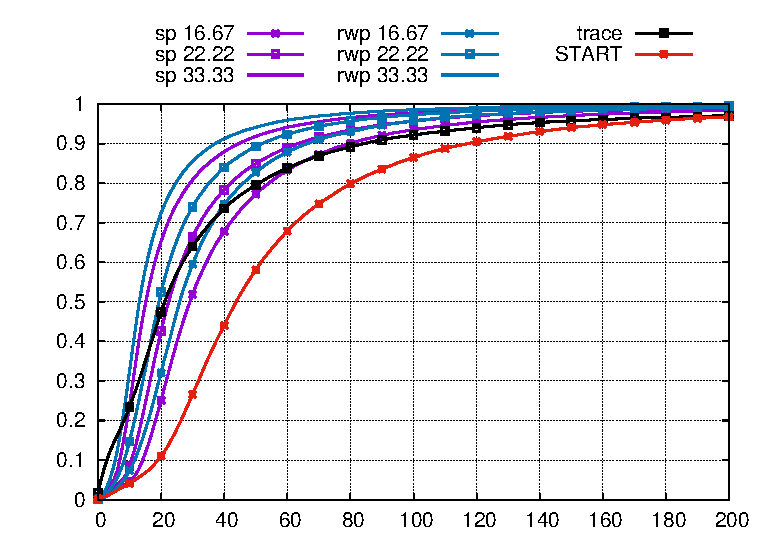
\includegraphics[width=0.24\textwidth]{figures_201103/Evaluation/contact/ct1000_6.eps}}
\subfigure[3000 nodes from 11:00 to 13:00]{\includegraphics[width=0.24\textwidth]{figures_201103/Evaluation/contact/ct3000_11.eps}}
\subfigure[3000 nodes from 17:00 to 19:00]{\includegraphics[width=0.24\textwidth]{figures_201103/Evaluation/contact/ct3000_17.eps}}
\subfigure[3000 nodes from 22:00 to 24:00]{\includegraphics[width=0.24\textwidth]{figures_201103/Evaluation/contact/ct3000_22.eps}}
\caption{Contact times distribution}\label{figure_contact_ct}
\end{figure*}

\begin{figure*}[!t]
\centering
\subfigure[1000 nodes from 6:00 to 8:00]{\includegraphics[width=0.24\textwidth]{figures_201103/Evaluation/contact/ict1000_6.eps}}
\subfigure[3000 nodes from 11:00 to 13:00]{\includegraphics[width=0.24\textwidth]{figures_201103/Evaluation/contact/ict3000_11.eps}}
\subfigure[3000 nodes from 17:00 to 19:00]{\includegraphics[width=0.24\textwidth]{figures_201103/Evaluation/contact/ict3000_17.eps}}
\subfigure[3000 nodes from 22:00 to 24:00]{\includegraphics[width=0.24\textwidth]{figures_201103/Evaluation/contact/ict3000_22.eps}}
\caption{Inter-contact times distribution }\label{figure_contact_ict}
\end{figure*}

\begin{figure*}[!t]
\centering
\subfigure[1000 nodes from 6:00 to 8:00]{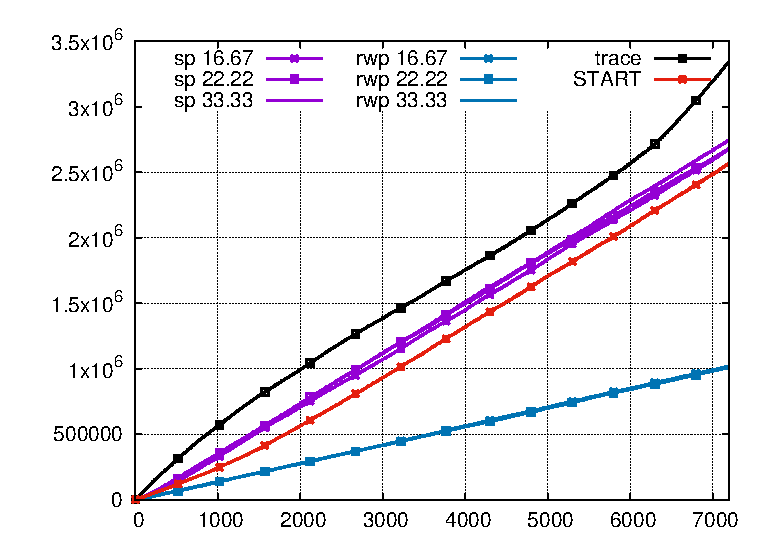
\includegraphics[width=0.24\textwidth]{figures_201103/Evaluation/contact/tc1000_6.eps}}
\subfigure[3000 nodes from 11:00 to 13:00]{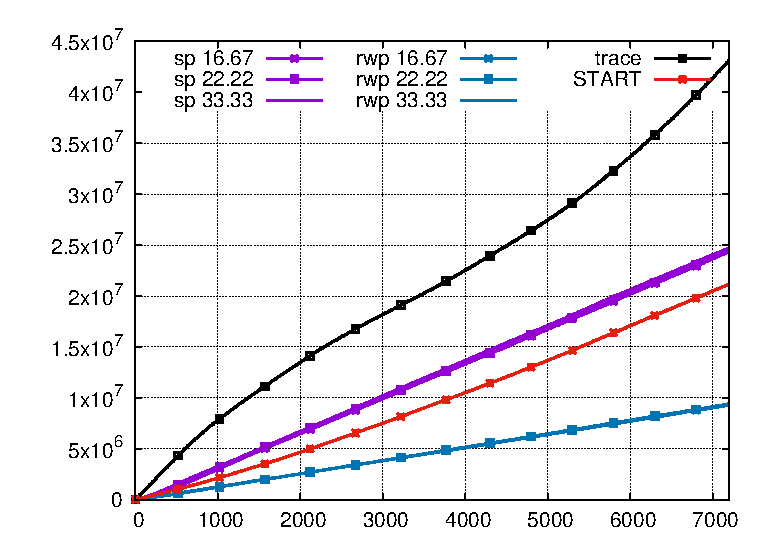
\includegraphics[width=0.24\textwidth]{figures_201103/Evaluation/contact/tc3000_11.eps}}
\subfigure[3000 nodes from 17:00 to 19:00]{\includegraphics[width=0.24\textwidth]{figures_201103/Evaluation/contact/tc3000_17.eps}}
\subfigure[3000 nodes from 22:00 to 24:00]{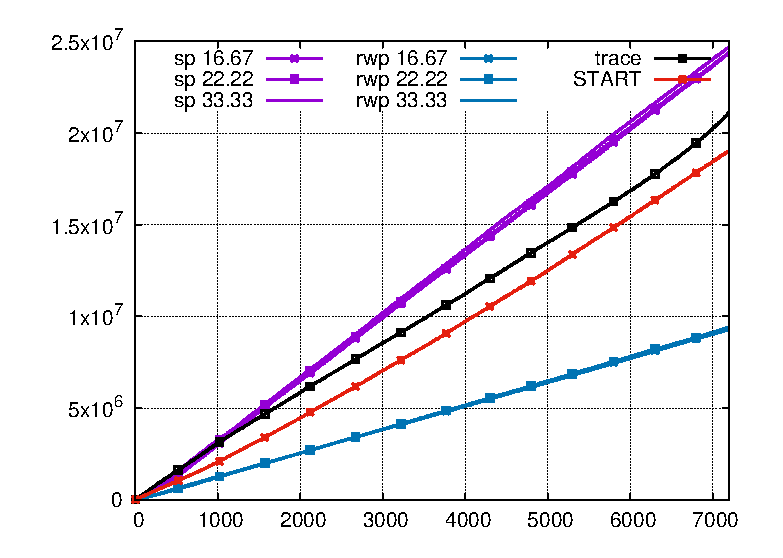
\includegraphics[width=0.24\textwidth]{figures_201103/Evaluation/contact/tc3000_22.eps}}
\caption{Time vs. total contact time.}\label{figure_contact_ct}
\end{figure*}


Contact defines an opportunity to communicate, a contact range should be assigned to quantify the max distance we consider two nodes contact with each other. 
In our simulations, the transmit ranges of high-speed interfaces and blue tooth interface are both set to $200m$ for potential contacts. 

The contact time and inter contact time among vehicles are also evaluated as the indicators to validate the similarity.
Fig. \ref{figure_contact_ct} and fig. \ref{figure_contact_ict} reports the contact time and inter-contact distributions, which shows the probability of the contact or inter-contact time smaller than certain time length. To substantiate, a point $(25,0.5)$ in the plots means the probability is $0.5$ when contact or inter-contact time is shorter than $25s$. 
%Clearly, START matches the real traces best among three mobility models.
From fig. \ref{figure_contact_ct} the speed will effect the contact distribution of SP and RWP. The speed in a low speed range will makes the contact time distribution of SP and RWP approach that of real traces. For START, in the time from 17:00 to 19:00, the model matches with the real traces best. 
Fig. \ref{figure_contact_ict} also show the sum of contact time regarding to the simulation time.
For the inter contact time, the curves of SP (RWP) are close with each other, which means the speed range dose not make much difference on the inter contact time. Compared with the distribution of contact time, it may because that the inter contact time are much longer than the contact time, the inter contact time is more stable to present the performance of nodes. 
In Fig. \ref{figure_total_contact_time}(a), the three purple lines of SP and the three blue lines of RWP are overlapping with each other, too.
The curves of the total contact time vs. time present a liner law. 
From the analysis above, for SP and RWP, the differences of speed ranges show little influence on these curves. 
%Clearly, the rank of the contact characteristic similarity with the real data is START $>$ SP $>$ RWP. 

To conclude, by comparing the node distribution and contact characteristics, the evaluation results confirm that START mobility model achieves great similarities with the real data. START takes the usage of speed and geographic features related with taxi status, while SP employs the map information and RWP is a random model taking use of no realistic data.

